\documentclass[12pt]{article}
\usepackage{pdfpages}

\begin{document}
\title{Math in Decision Making\\ Unit on Topology:\\ 
Picture Hanging Puzzles\\ and\\ Knot Theory}
\author{Instructor: Theron J Hitchman}
\date{Spring 2015}

\maketitle

Our first topic of study is some \emph{topology}. The particular questions we will take up are in \emph{knot theory}, with a short lead-in by way of \emph{picture hanging puzzles}. If none of those words is familiar to you, do not worry. We will sort them out soon.

For each class meeting in this unit, please read the corresponding section here and work out the associated exercises. Students are expected to come to class prepared, and this includes having made an honest effort to solve all the exercises before class. The readings are not long (the shortest is two pages and the longest is about six pages) but they might take some time to sink in, and some effort and thinking will be required in the exercises.

\newpage
$\phantom{Theron J Hitchman}$
\newpage
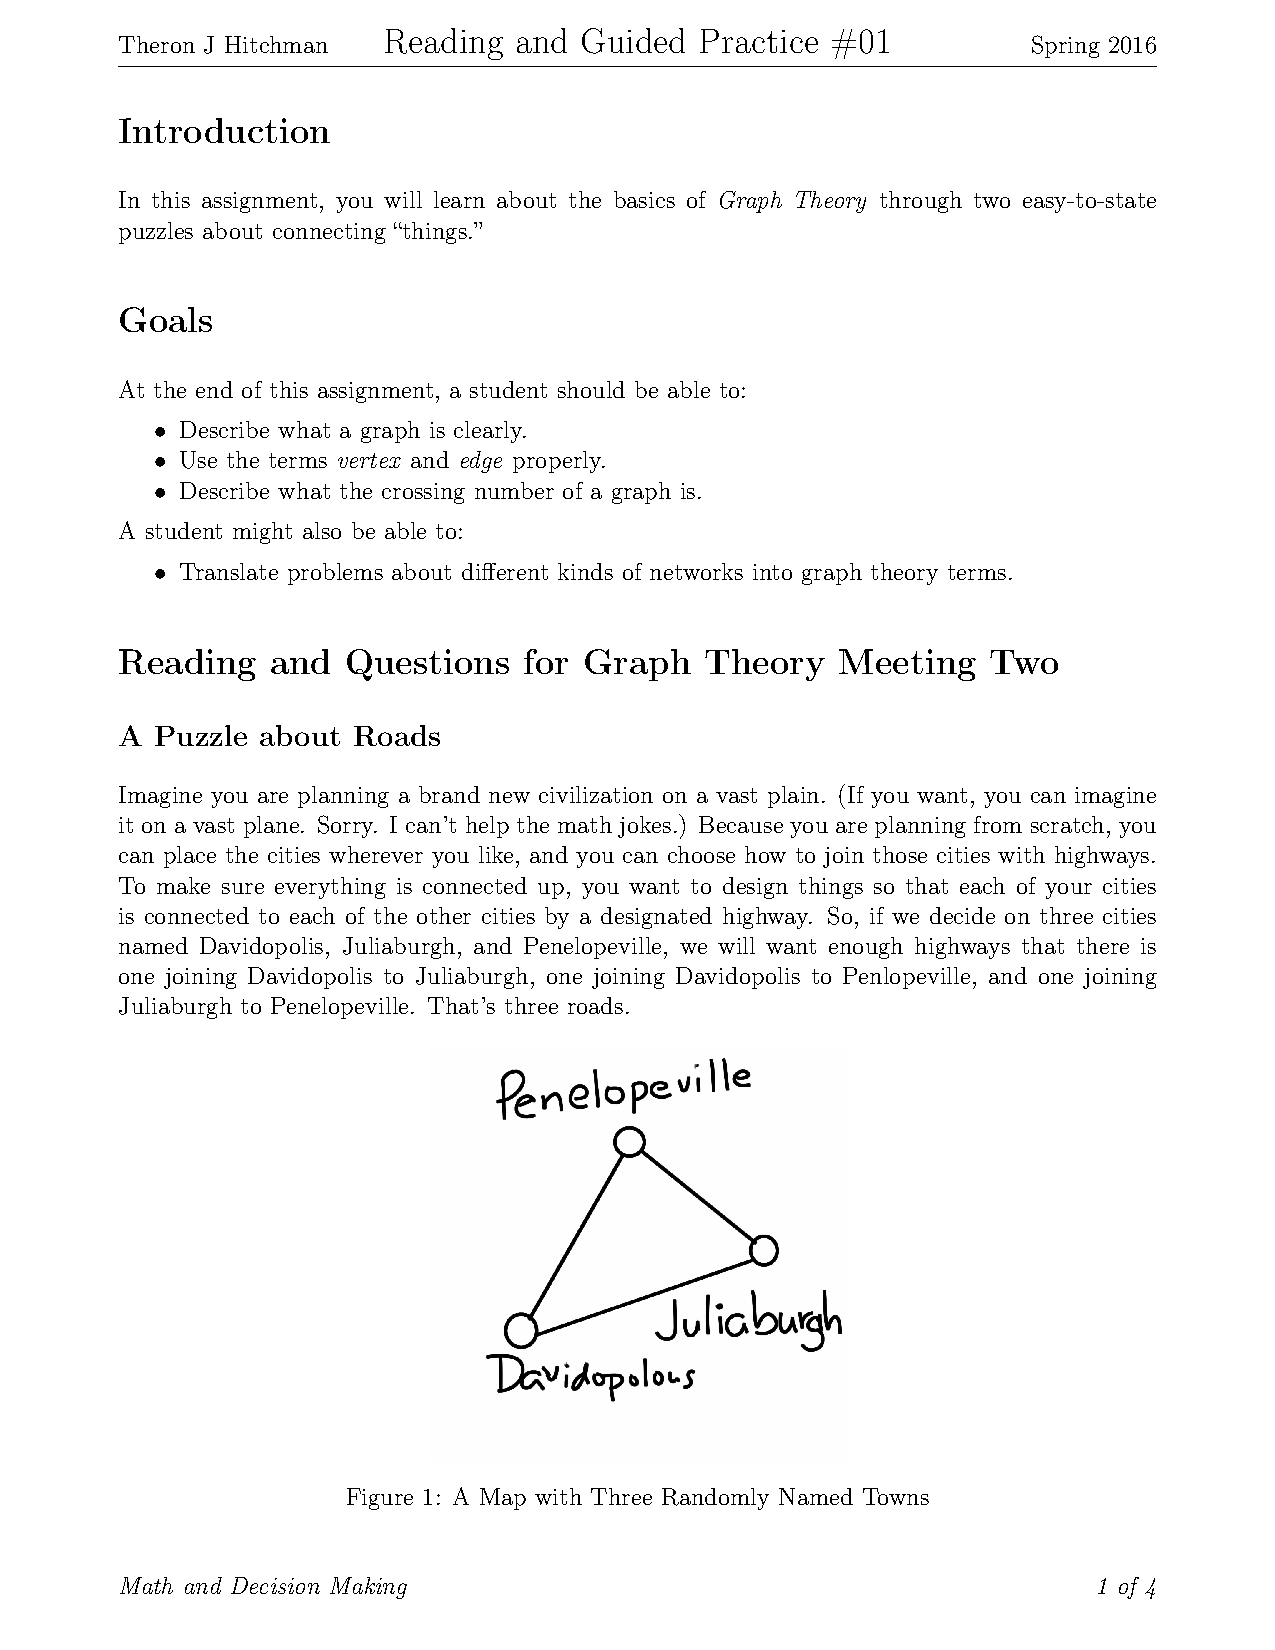
\includepdf[pages=-]{rgp01.pdf}
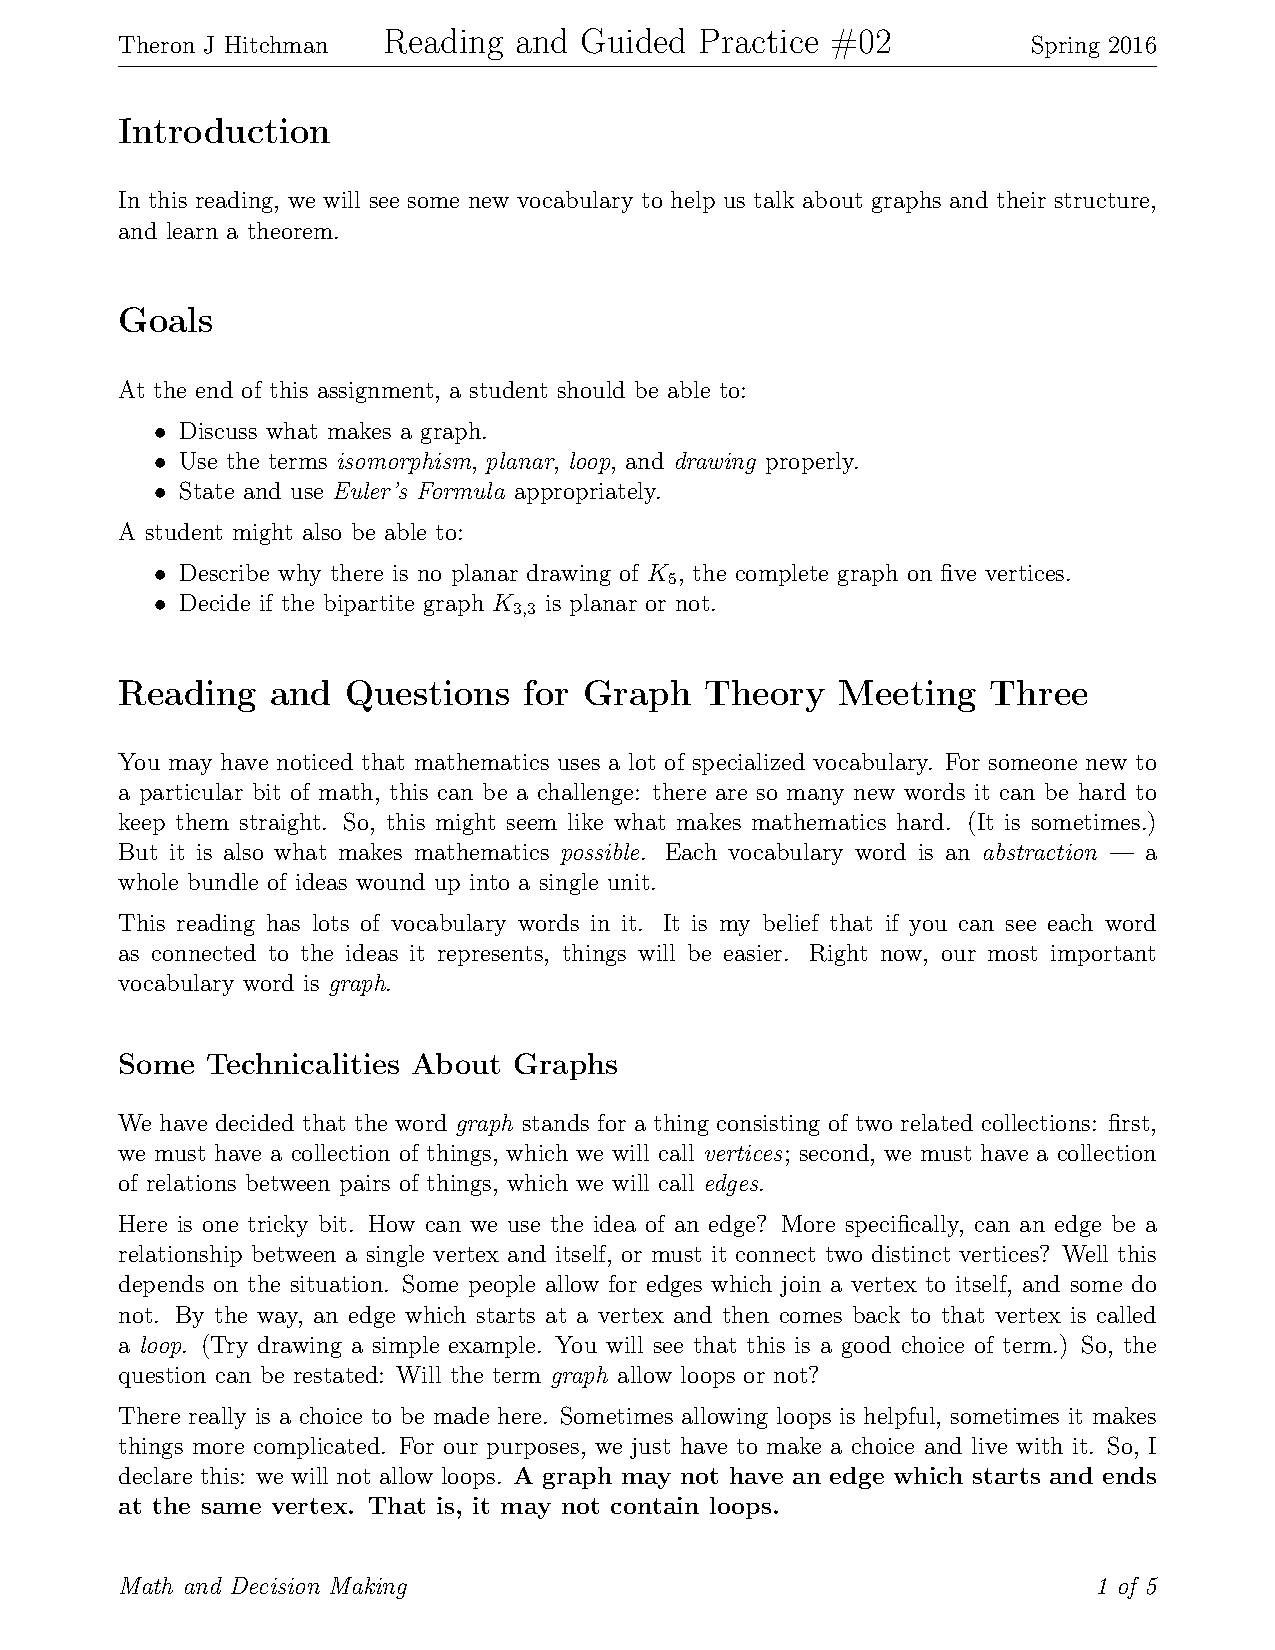
\includepdf[pages=-]{rgp02.pdf}
{\Huge \textbf{STOP}}\\[1in]

Don't read on, yet. If you are curious, go back and reread. Go deeper.
\newpage
$\phantom{Theron J Hitchman}$
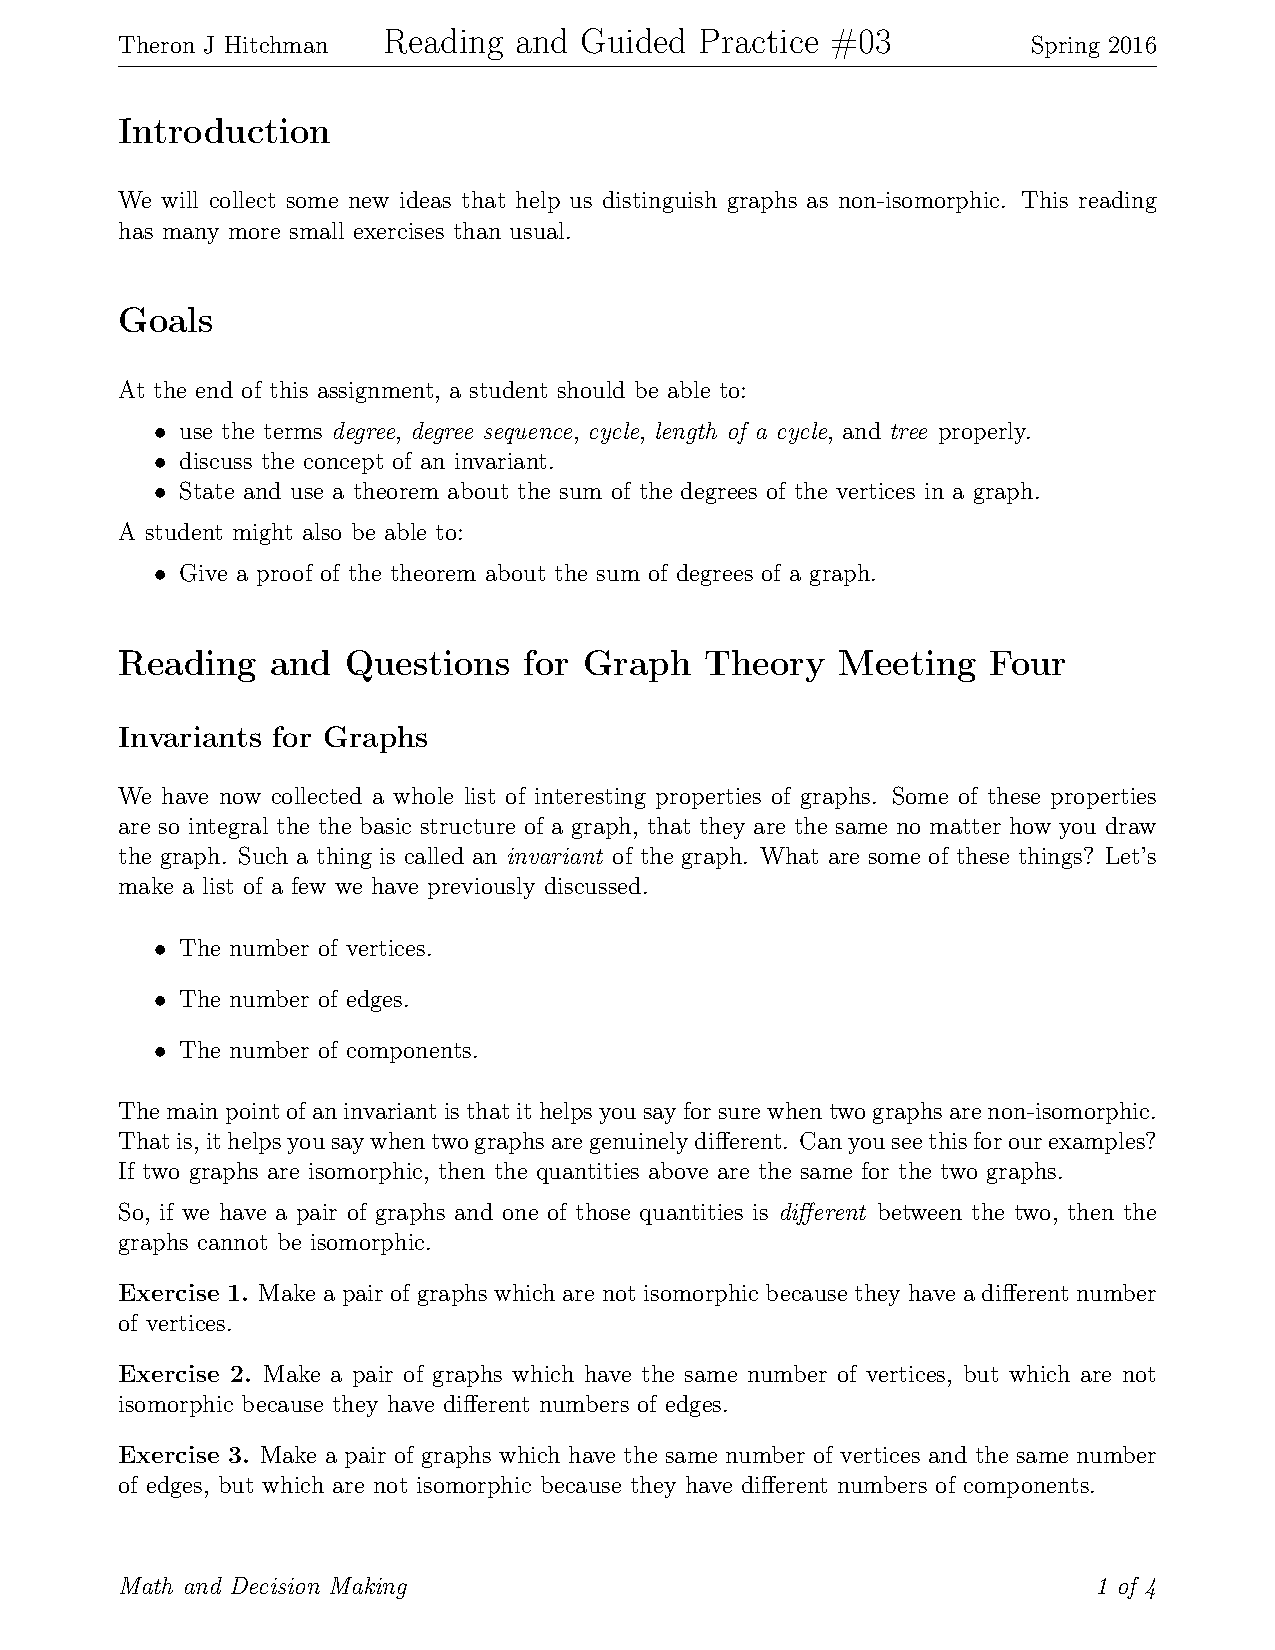
\includepdf[pages=-]{rgp03.pdf}
\newpage
$\phantom{Theron J Hitchman}$
\newpage
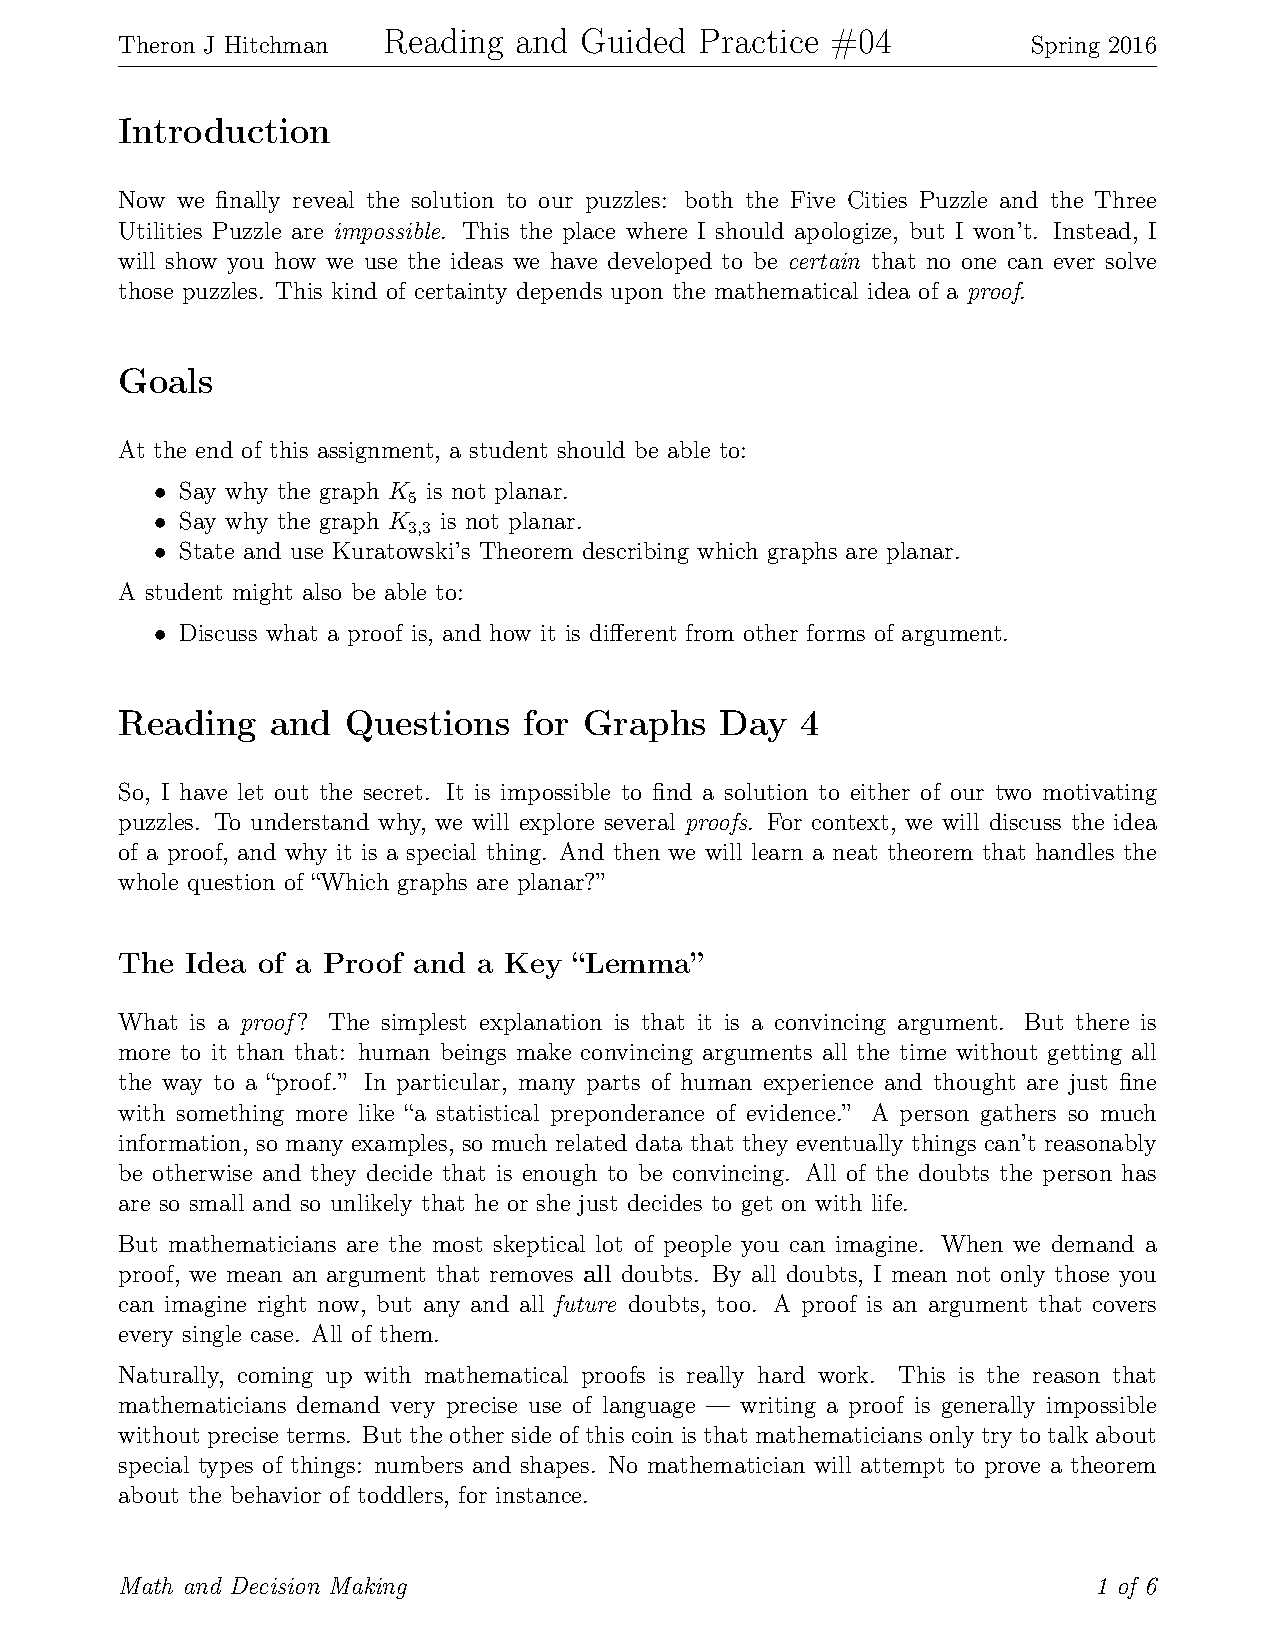
\includepdf[pages=-]{rgp04.pdf}
\newpage
$\phantom{Theron J Hitchman}$
\newpage
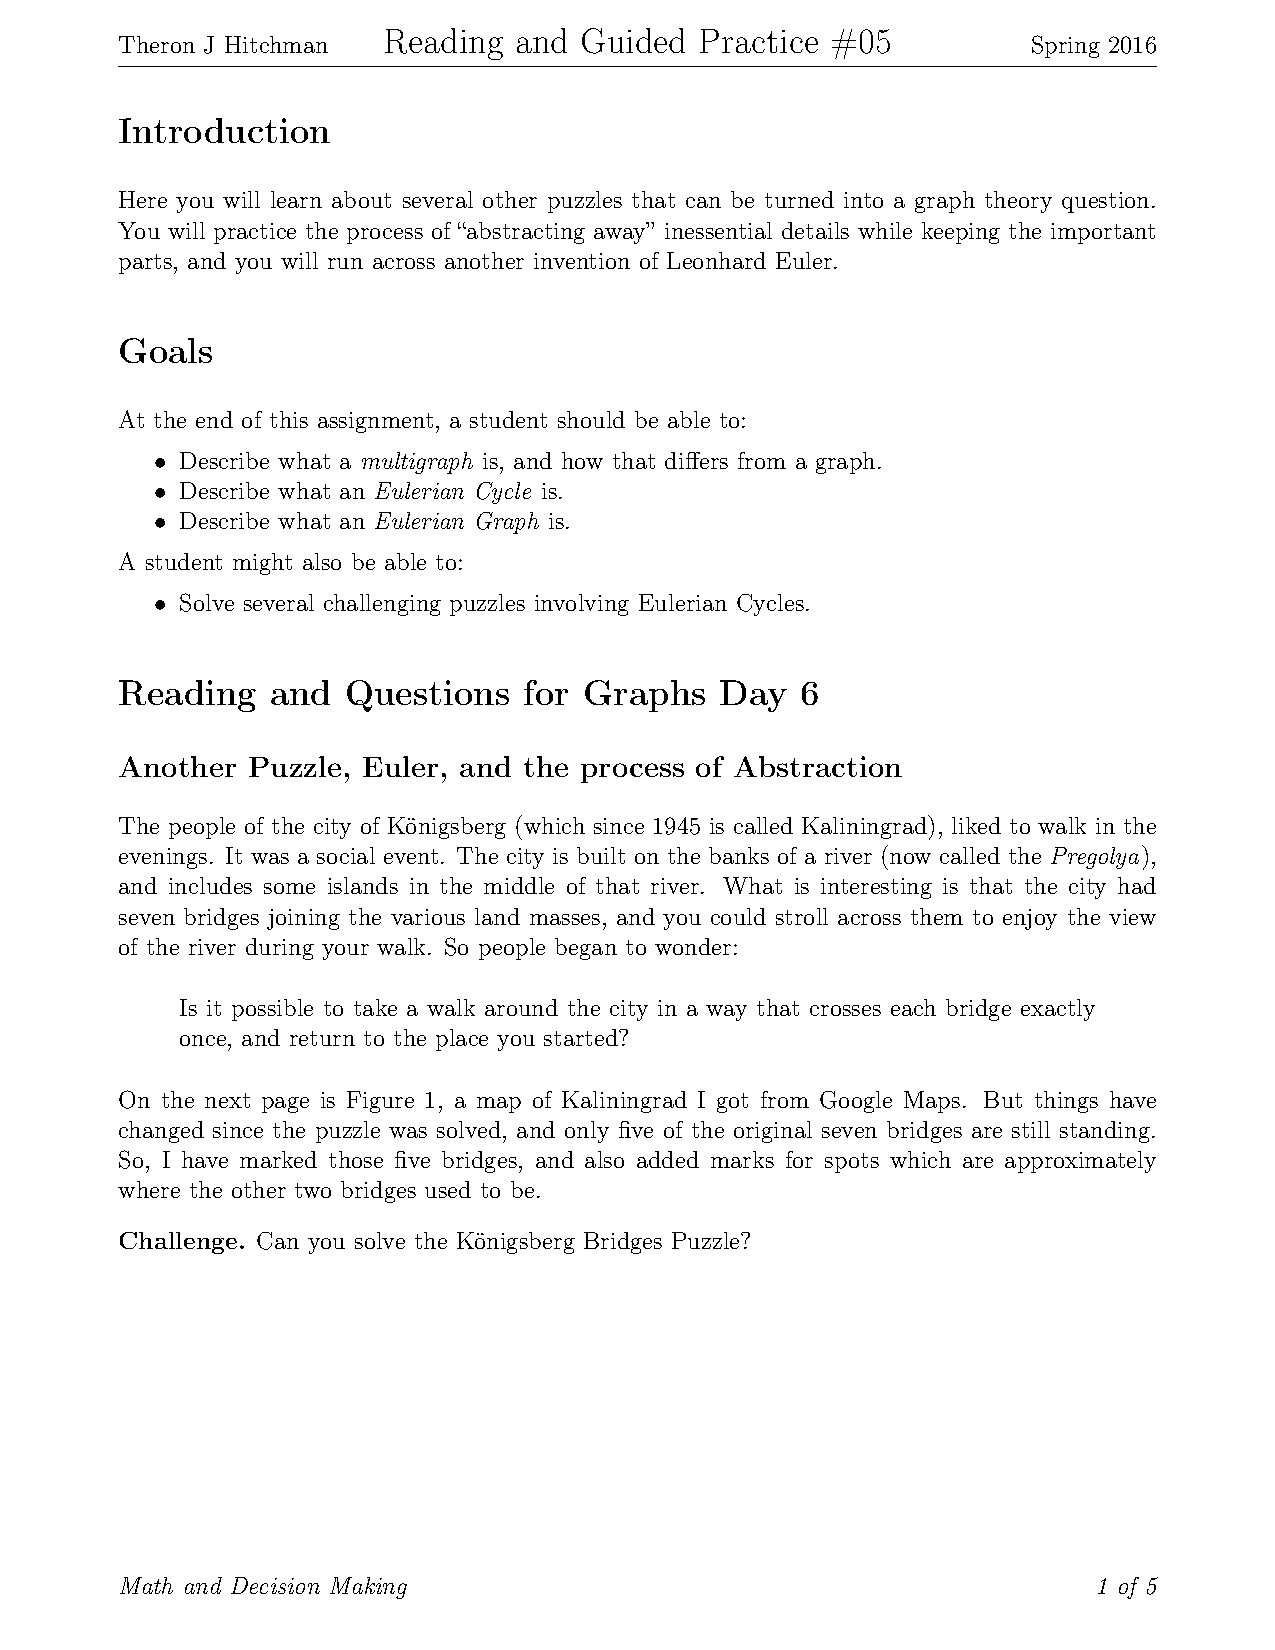
\includepdf[pages=-]{rgp05.pdf}
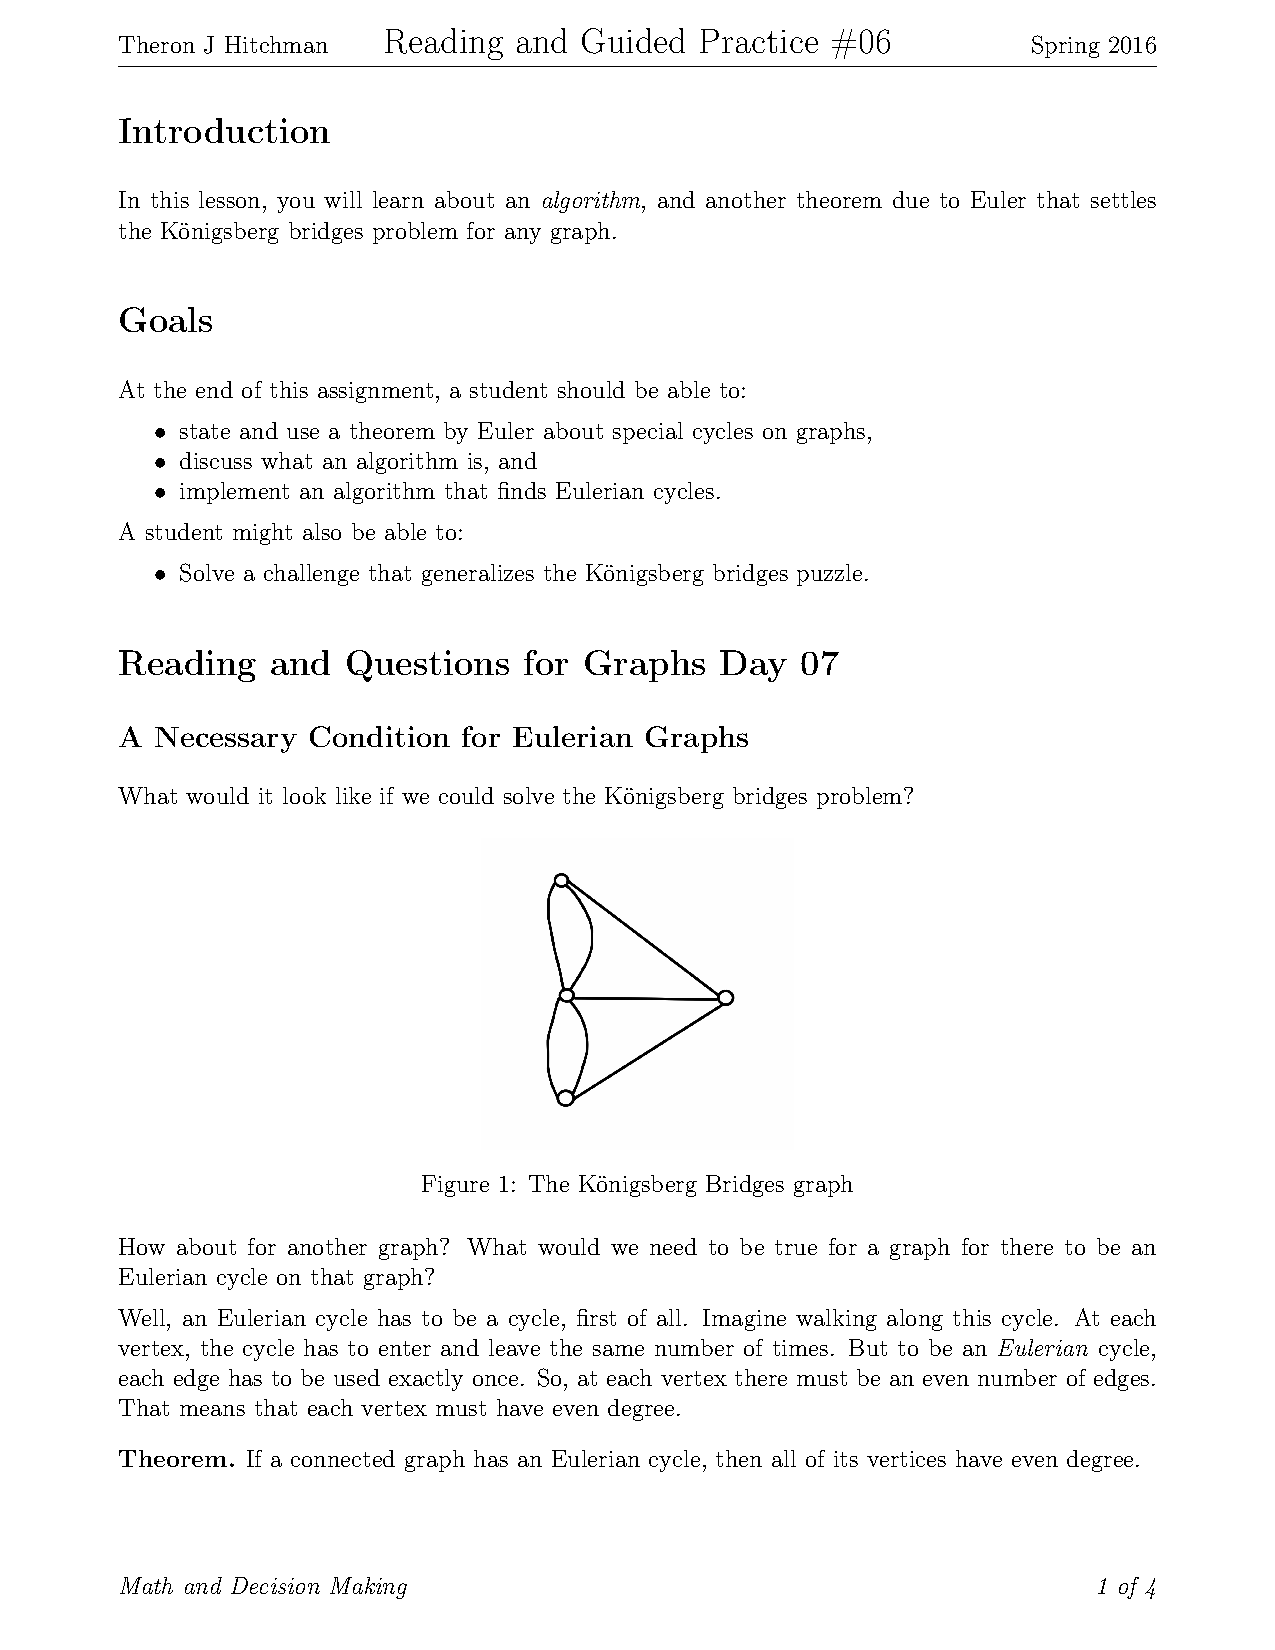
\includepdf[pages=-]{rgp06.pdf}
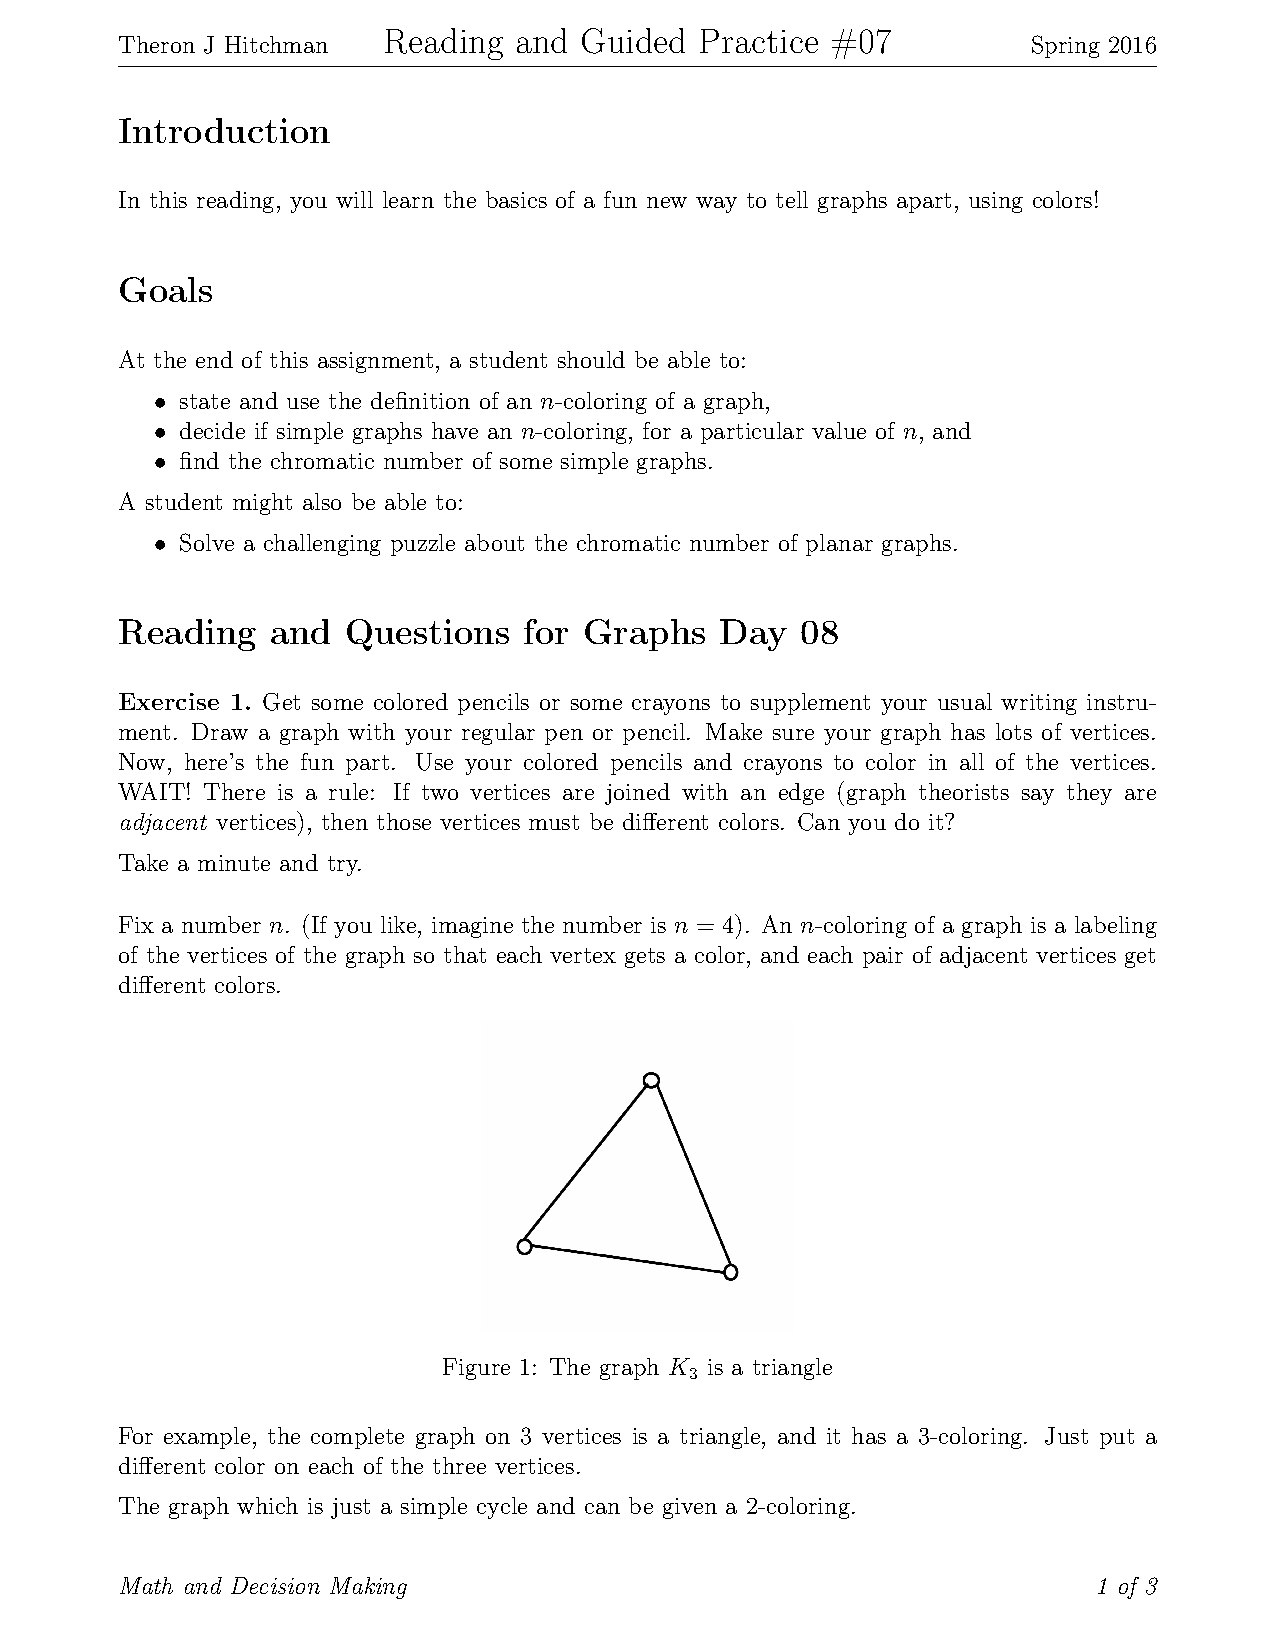
\includepdf[pages=-]{rgp07.pdf}
\newpage
$\phantom{Theron J Hitchman}$
\newpage
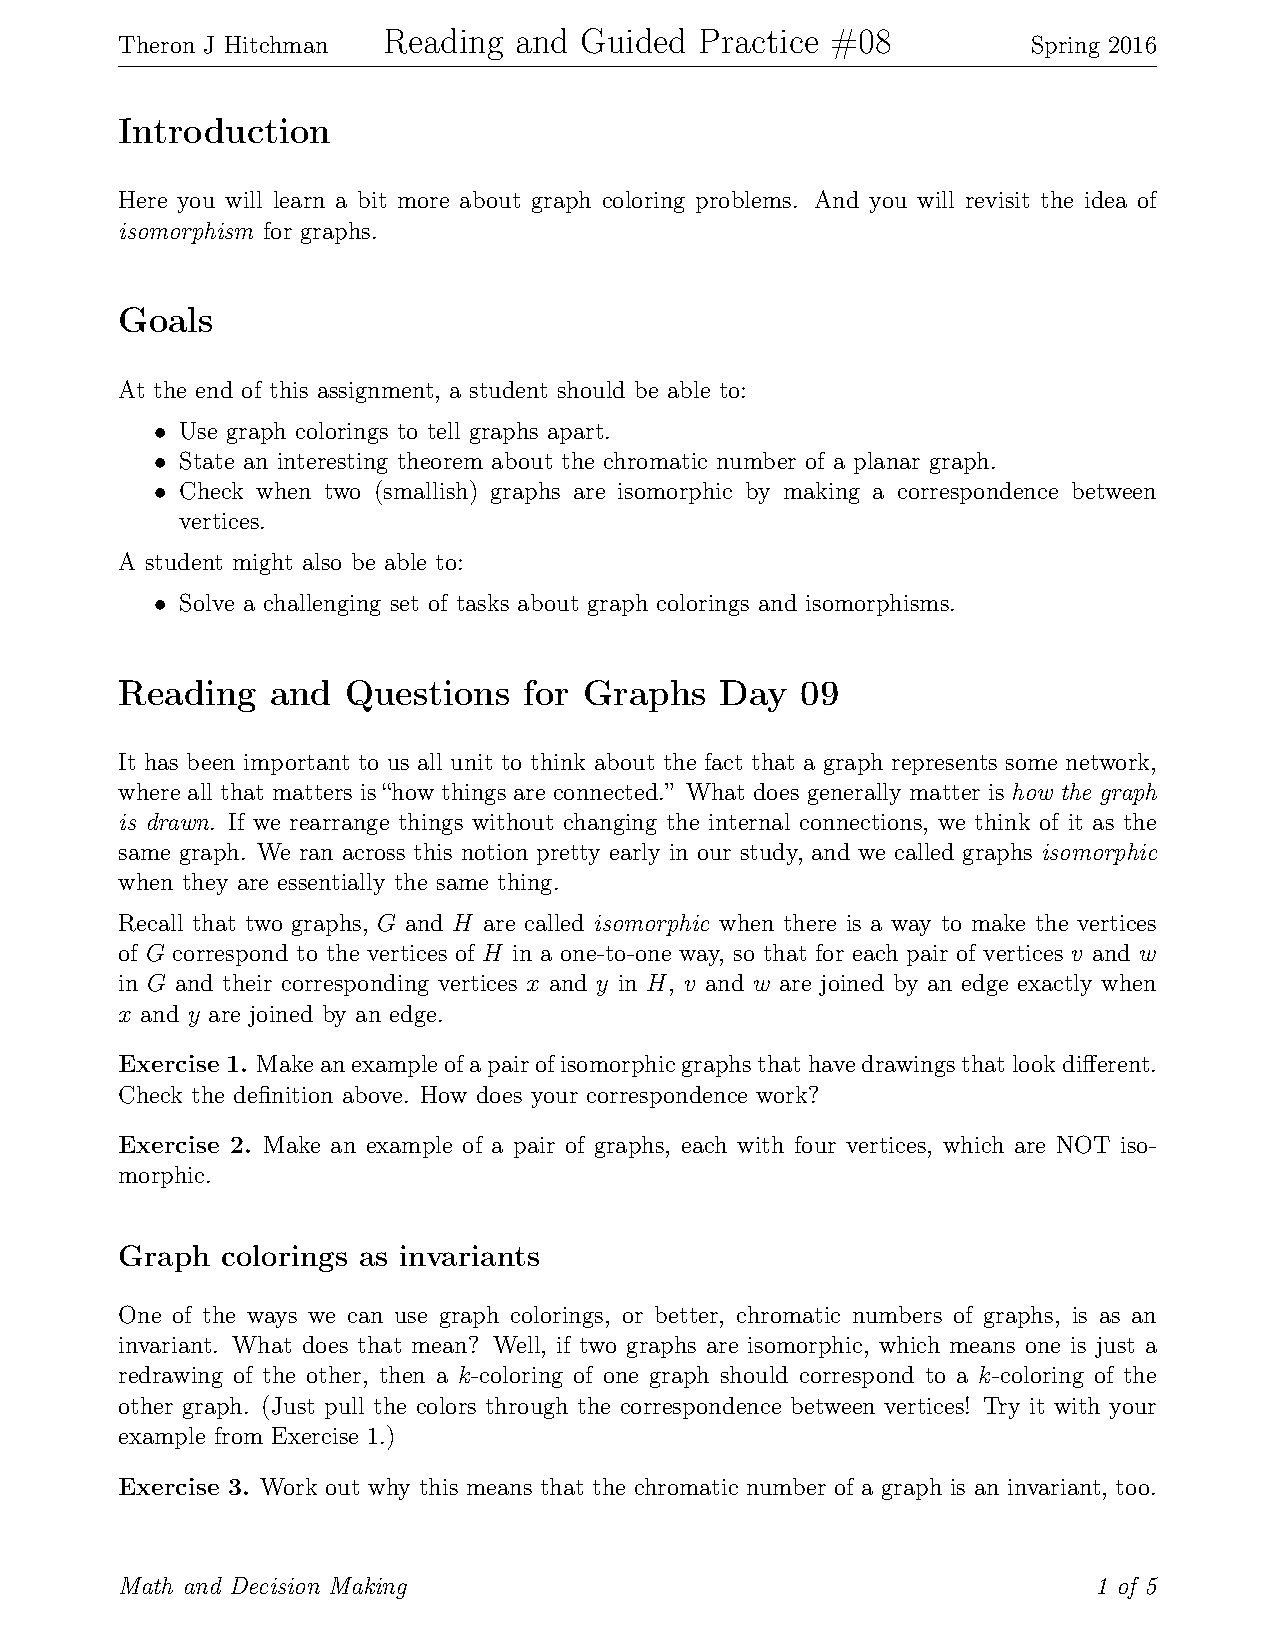
\includepdf[pages=-]{rgp08.pdf}
\newpage
$\phantom{Theron J Hitchman}$
\newpage
\includepdf[pages=-]{rgp09.pdf}
\newpage
$\phantom{Theron J Hitchman}$
\newpage
\includepdf[pages=-]{rgp10.pdf}
\includepdf[pages=-]{rgp11.pdf}
\includepdf[pages=-]{rgp12.pdf}

\end{document}